\fontfamily{\sfdefault}\selectfont
% XCircuit output "simulator.tex" for LaTeX input from simulator.ps
\def\putbox#1#2#3#4{\makebox[0.00000in][l]{\makebox[#1][l]{}\raisebox{\baselineskip}[0.00000in][0.00000in]{\raisebox{#2}[0.00000in][0.00000in]{\scalebox{#3}{#4}}}}}
\def\rightbox#1{\makebox[0.00000in][r]{#1}}
\def\centbox#1{\makebox[0.00000in]{#1}}
\def\topbox#1{\raisebox{-0.60\baselineskip}[0.00000in][0.00000in]{#1}}
\def\midbox#1{\raisebox{-0.20\baselineskip}[0.00000in][0.00000in]{#1}}
   \scalebox{1}{
   \normalsize
   \parbox{6.25002in}{
   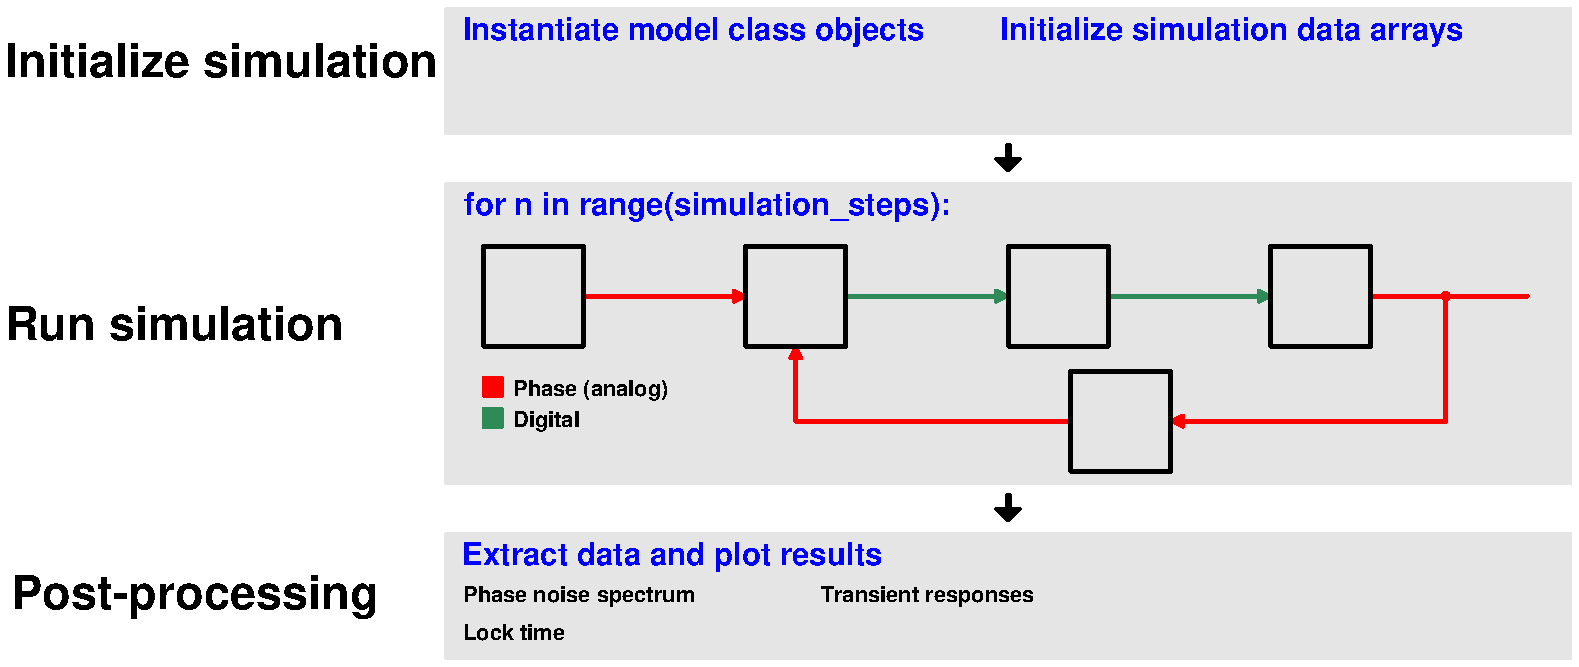
\includegraphics[scale=0.60000]{./figs/simulator.pdf}\\
   % translate x=1040 y=384 scale 0.38
   \putbox{3.08400in}{1.45800in}{0.84}{\texttt{tdc}}%
   \putbox{4.38600in}{0.96000in}{0.84}{\texttt{div}}%
   \putbox{4.15800in}{1.45800in}{0.84}{\texttt{lf}}%
   \putbox{5.18400in}{1.45800in}{0.84}{\texttt{dco}}%
   \putbox{2.03400in}{1.45800in}{0.84}{\texttt{clk}}%
   \putbox{3.48600in}{1.03200in}{0.84}{\texttt{div\_sig[n]}}%
   \putbox{2.38200in}{1.56000in}{0.84}{\texttt{clk\_sig[n]}}%
   \putbox{3.43200in}{1.53600in}{0.84}{\texttt{tdc\_sig[n]}}%
   \putbox{4.48200in}{1.53600in}{0.84}{\texttt{lf\_sig[n]}}%
   \putbox{5.53200in}{1.53600in}{0.84}{\texttt{dco\_sig[n]}}%
   \putbox{4.00800in}{2.35800in}{0.84}{\texttt{clk\_sig[n]}}%
   \putbox{4.00800in}{2.20800in}{0.84}{\texttt{tdc\_sig[n]}}%
   \putbox{4.71000in}{2.35800in}{0.84}{\texttt{lf\_sig[n]}}%
   \putbox{4.71000in}{2.20800in}{0.84}{\texttt{dco\_sig[n]}}%
   \putbox{5.38200in}{2.35800in}{0.84}{\texttt{div\_sig[n]}}%
   \putbox{1.86000in}{2.35800in}{0.84}{\texttt{clk}}%
   \putbox{1.86000in}{2.20800in}{0.84}{\texttt{tdc}}%
   \putbox{2.40600in}{2.35800in}{0.84}{\texttt{lf}}%
   \putbox{2.40600in}{2.20800in}{0.84}{\texttt{dco}}%
   \putbox{2.95800in}{2.35800in}{0.84}{\texttt{div}}%
   \putbox{1.88400in}{0.83400in}{0.84}{t$_{sim}$ = \texttt{n}$\Delta$t}%
   } % close 'parbox'
   } % close 'scalebox'
   \vspace{-\baselineskip} % this is not necessary, but looks better
\fontfamily{\rmdefault}\selectfont
